\section{Experiments}
In this section,  We compare PINS with state-of-the-art pruning algorithms and perform detailed analysis  to understand the effectiveness of PINS.
\subsection{Setup}
\subsubsection{Tasks}
We conduct experiments on a comprehensive spectrum of tasks following standard data splits. \\
\textbf{Natural Language Understanding. } We opt for tasks from the GLUE~\cite{glue} benchmark, including linguistic acceptability~(CoLA), natural language inference~(RTE, QNLI, MNLI), paraphrase~(MRPC, QQP), sentiment analysis~(SST-2) and textual similarity~(STS-B). Because the official test set of GLUE is hidden, we randomly split a small portion of training set as validation set and treat the original validation set as test set. \\
\textbf{Question Answering. } We use SQuAD v1.1~\cite{squad} as a representative dataset for extractive question answering following previous work~\cite{platon}. \\
\textbf{Named Entity Recognition. } We also examine our approach on CoNLL 2003~\cite{conll2003} for token-level named entity recognition task. \\
\textbf{Data-to-Text Generation.} Besides language understanding tasks, we also extend our evaluation to data-to-text generation on three datasets: E2E~\cite{e2e}, DART~\cite{dart}, and WebNLG~\cite{webnlg}, which involves generating a piece of fluent text from  a set of structured relational triples. \\



\subsubsection{Baselines}
\textbf{Magnitude-based.} Iterative magnitude pruning~(IMP)~\cite{gupta} is the state-of-the-art magnitude-based approach.

\noindent
\textbf{Sensitivity-based.} $l_0$-regularization~\cite{l0} trains masking variables via re-parametrization trick with $l_0$ penalty; SMvP~\cite{movement} uses accumulated sensitivity as importance metric; PST~\cite{pst} proposed a hybrid importance criterion combining both magnitude and sensitivity; PLATON~\cite{platon} uses a modified variant of sensitivity by exponential moving average and uncertainty re-weighting.

%\subsubsection{Models}

\begin{table*}[t]
	\centering
	\normalsize
	\small
	\begin{tabular}{c|l|cccccccc|c}
		\toprule
		\multirow{2}{*}{Sparsity} & \multicolumn{1}{c|}{\multirow{2}{*}{Method}} & \multicolumn{1}{c}{\multirow{2}{*}{\begin{tabular}[c]{@{}c@{}}\textbf{RTE}\\ Acc\end{tabular}}} & \multicolumn{1}{c}{\multirow{2}{*}{\begin{tabular}[c]{@{}c@{}}\textbf{MRPC}\\ F1\end{tabular}}} & \multicolumn{1}{c}{\multirow{2}{*}{\begin{tabular}[c]{@{}c@{}}\textbf{STS-B}\\ Pearson\end{tabular}}} & \multicolumn{1}{c}{\multirow{2}{*}{\begin{tabular}[c]{@{}c@{}}\textbf{CoLA}\\ Mcc\end{tabular}}} & \multicolumn{1}{c}{\multirow{2}{*}{\begin{tabular}[c]{@{}c@{}}\textbf{SST-2}\\ Acc\end{tabular}}} & \multicolumn{1}{c}{\multirow{2}{*}{\begin{tabular}[c]{@{}c@{}}\textbf{QNLI}\\ Acc\end{tabular}}} & \multicolumn{1}{c}{\multirow{2}{*}{\begin{tabular}[c]{@{}c@{}}\textbf{MNLI}\\ Acc\end{tabular}}} & \multicolumn{1}{c|}{\multirow{2}{*}{\begin{tabular}[c]{@{}c@{}}\textbf{QQP}\\ Acc\end{tabular}}} & \multicolumn{1}{c}{\multirow{2}{*}{Avg.}}\\
		& \multicolumn{1}{c|}{}                        & \multicolumn{1}{c}{}                                                                   & \multicolumn{1}{c}{}                                                                   & \multicolumn{1}{c}{}                                                                    & \multicolumn{1}{c}{}                                                                     & \multicolumn{1}{c}{}                                                                    & \multicolumn{1}{c}{}                                                                    & \multicolumn{1}{c}{}             & \multicolumn{1}{c|}{}                &\multicolumn{1}{c}{}                                                  \\
		\midrule
		\multicolumn{1}{c|}{0\%}   & Fine-tune$\dagger$                                   & 69.3                                                                                   &
		90.3                                                                            & 90.2       & 58.3                                                                                    & 92.4                                                                                     & 91.3                                                                                    & 84.0                                                                                    & 91.5                                 &  83.4                                                \\
		\midrule
		\multirow{6}{*}{80\%}     &IMP$\dagger$                                                 &65.7                                                                                        &86.2                                                                               & 86.8        & 42.5                                                                                        &84.3                                                                                 &89.2                                                                                     &82.2                                                                                        &  86.0                                                    &    77.9                              \\
		&$l_0$-regularization$\dagger$                                                 & 63.2                                                                                       & 80.2                                                                                 & 82.8      &0.0                                                                                         &   85.0                                                                                       &       85.0                                                                                  &    80.8                                                                                     &  88.5                                                          &  70.7                          \\
		&SMvP$\dagger$                                                 &62.8                                                                                        &   86.7                                                                    & 87.8                 & 48.5                                                                                        &89.0                                                                                          &  88.3                                                                                       &   81.9                                                                                      &    90.6                                                                 & 79.5                  \\
		&PST                                             &          63.0                                                                              &       87.4   & 88.0                                                                              &      44.6                                                                                   &  89.3                                                                                        &    88.3                                                                                     &    79.3                                                                                     &  88.9                                                                    &  78.6                \\
		&PLATON$\dagger$                                             &   68.6                                                                                     & 89.8                                                                                    &89.0   &     54.5                                                                                    & 91.2                                                                                         &   90.1                                                                                      &    83.3                                                                                     &    90.7                                                                 &82.2                   \\
		&PINS~(ours)                                             &\textbf{72.7}                                                                                       &\textbf{90.9}                                                                                      &\textbf{89.2}   & \textbf{57.1}                                                                                      & \textbf{91.9}                                                                                       &\textbf{91.2}                                                                                         &  \textbf{83.9}                                                                                      &  \textbf{90.9}                                                                    & \textbf{83.5}               \\
		\midrule
		\multirow{6}{*}{90\%}     &IMP$\dagger$                                                 &57.4                                                                                       &80.3                                                                           &83.4             & 18.3                                                                                        &  80.7                                                                                        & 86.6                                                                                        &78.9                                                                                         &78.8                                                                     &  70.5                 \\
		&$l_0$-regularizatio$\dagger$                                                 &59.9                                                                                        &  79.5                                                                               &  82.7     & 0.0                                                                                        &    82.5                                                                                      &   82.8                                                                                      &    78.4                                                                                     &   87.6                                                                           &69.1          \\
		&SMvP$\dagger$                                                 &58.8                                                                                        &   85.9                                                                                &86.5     &  0.0                                                                                       &   87.4                                                                                       &  86.6                                                                                       &  80.9                                                                                       &    90.2                                                                        &  72.1          \\
		&PST$\ddagger$                                             &62.8                                                                                        &  85.6                                                                             &81.7         & 42.5                                                                                        & 88.7                                                                                         &   86.0                                                                                      &    76.7                                                                                     & 83.9                                                                              & 76.0        \\
		& PLATON$\dagger$                                                &  65.3                                                                                      & 88.8                                                                               &87.4        &44.3                                                                                         &  90.5                                                                                        &88.9                                                                                         &  81.8                                                                                       &  90.2                                                                              &   79.6     \\
		&PINS~(ours)                                             &  \textbf{68.5}                                                                                      & \textbf{90.1}                                                                              &\textbf{87.9}         & \textbf{49.8}                                                                                        &  \textbf{91.0}                                                                                        &  \textbf{89.5}                                                                                       &   \textbf{82.7}                                                                                      &  \textbf{90.6}                                   & \textbf{81.3}            \\
		\bottomrule                                     
	\end{tabular}
	\caption{Results with BERT$_{\text{base}}$ on the GLUE development set. For MNLI, the results are averaged on MNLI-m and MNLI-mm. $\dagger$ indicates the results are directly quoted from \citet{platon} while $\ddagger$ indicates the results are reported by \citet{pst}. }
	\label{table:glue}
\end{table*}

\subsubsection{Implementation Details}
We mainly conduct experiments on the pre-trained BERT$_{\text{base}}$~\cite{bert} as a pruning target for all tasks except data-to-text generation. We defer the pruning results of MiniLM$_{\text{12L-384H}}$~\cite{minilm} and Electra$_{\text{base}}$~\cite{electra} to Appendix \ref{sec:A}. For data-to-text generation, we adopt the pre-trained GPT-2~\cite{gpt2} following 
a prior study~\cite{pst}.

During pruning, we employ the cubic sparsity scheduler~\cite{movement,platon} to gradually increase the sparsity level from 0 to the specified target sparsity. To avoid tremendous computation cost brought by hyper-parameter tuning, we only search the batch size from $\{16,32\}$ and fix the learning rate as 3e-5 for all experiments on GLUE and CoNLL. For SQuAD v1.1, we fix the batch size as 16 and the learning rate as 3e-5 following \citet{platon}. We adopt AdamW~\cite{adamw} as the default optimizer.
To reduce the variance induced by mini-batch sampling, we adopt a smoothing technique similar to PLATON. We run each experiment five times with different random seeds and report the average results~(significance tests with $p$-value~<~0.05 are conducted  for  all performance gains).

\subsection{Main Results}


% \begin{table*}[t]
% 	\centering
% 	\normalsize
% 	\small
% 	\begin{tabular}{c|l|ccccccc|c}
% 		\toprule
% 		\multirow{2}{*}{Sparsity} & \multicolumn{1}{c|}{\multirow{2}{*}{Method}} & \multicolumn{1}{c}{\multirow{2}{*}{\begin{tabular}[c]{@{}c@{}}\textbf{RTE}\\ Acc\end{tabular}}} & \multicolumn{1}{c}{\multirow{2}{*}{\begin{tabular}[c]{@{}c@{}}\textbf{MRPC}\\ F1\end{tabular}}} & \multicolumn{1}{c}{\multirow{2}{*}{\begin{tabular}[c]{@{}c@{}}\textbf{CoLA}\\ Mcc\end{tabular}}} & \multicolumn{1}{c}{\multirow{2}{*}{\begin{tabular}[c]{@{}c@{}}\textbf{SST-2}\\ Acc\end{tabular}}} & \multicolumn{1}{c}{\multirow{2}{*}{\begin{tabular}[c]{@{}c@{}}\textbf{QNLI}\\ Acc\end{tabular}}} & \multicolumn{1}{c}{\multirow{2}{*}{\begin{tabular}[c]{@{}c@{}}\textbf{MNLI}\\ Acc\end{tabular}}} & \multicolumn{1}{c}{\multirow{2}{*}{\begin{tabular}[c]{@{}c@{}}\textbf{QQP}\\ Acc\end{tabular}}} & \multicolumn{1}{|c}{\multirow{2}{*}{Macro Avg.}}\\
% 		& \multicolumn{1}{c|}{}                        & \multicolumn{1}{c}{}                                                                   & \multicolumn{1}{c}{}                                                                   & \multicolumn{1}{c}{}                                                                    & \multicolumn{1}{c}{}                                                                     & \multicolumn{1}{c}{}                                                                    & \multicolumn{1}{c}{}                                                                    & \multicolumn{1}{c|}{}             & \multicolumn{1}{c}{}                                                              \\
% 		\midrule
% 		\multicolumn{1}{c|}{0\%}   & Fine-tune$\dagger$                                   & 69.3                                                                                   &
% 		90.3                                                                                   & 58.3                                                                                    & 92.4                                                                                     & 91.3                                                                                    & 84.0                                                                                    & 91.5                                 &  82.4                                                \\
% 		\midrule
% 		\multirow{6}{*}{80\%}     &IMP$\dagger$                                                 &65.7                                                                                        &86.2                                                                                        & 42.5                                                                                        &84.3                                                                                 &89.2                                                                                     &82.2                                                                                        &  86.0                                                    &    76.6                              \\
% 		&$l_0$-regularization$\dagger$                                                 & 63.2                                                                                       & 80.2                                                                                       &0.0                                                                                         &   85.0                                                                                       &       85.0                                                                                  &    80.8                                                                                     &  88.5                                                          &  69.0                          \\
% 		&SMvP$\dagger$                                                 &62.8                                                                                        &   86.7                                                                                     & 48.5                                                                                        &89.0                                                                                          &  88.3                                                                                       &   81.9                                                                                      &    90.6                                                                 & 78.3                  \\
% 		&PST                                             &          63.0                                                                              &       87.4                                                                                 &      44.6                                                                                   &  89.3                                                                                        &    88.3                                                                                     &    79.3                                                                                     &  88.9                                                                    &  77.3                \\
% 		&PLATON$\dagger$                                             &   68.6                                                                                     & 89.8                                                                                       &     54.5                                                                                    & 91.2                                                                                         &   90.1                                                                                      &    83.3                                                                                     &    90.7                                                                 &81.2                   \\
% 		&PINS~(ours)                                             &\textbf{72.7}                                                                                       &\textbf{90.9}                                                                                        & \textbf{57.1}                                                                                      & \textbf{91.9}                                                                                       &\textbf{91.2}                                                                                         &  \textbf{83.9}                                                                                      &  \textbf{90.9}                                                                    & \textbf{82.7}               \\
% 		\midrule
% 		\multirow{6}{*}{90\%}     &IMP$\dagger$                                                 &57.4                                                                                       &80.3                                                                                        & 18.3                                                                                        &  80.7                                                                                        & 86.6                                                                                        &78.9                                                                                         &78.8                                                                     &  68.7                 \\
% 		&$l_0$-regularizatio$\dagger$                                                 &59.9                                                                                        &  79.5                                                                                      & 0.0                                                                                        &    82.5                                                                                      &   82.8                                                                                      &    78.4                                                                                     &   87.6                                                                           &67.2          \\
% 		&SMvP$\dagger$                                                 &58.8                                                                                        &   85.9                                                                                     &  0.0                                                                                       &   87.4                                                                                       &  86.6                                                                                       &  80.9                                                                                       &    90.2                                                                        &  70.0          \\
% 		&PST$\ddagger$                                             &62.8                                                                                        &  85.6                                                                                      & 42.5                                                                                        & 88.7                                                                                         &   86.0                                                                                      &    76.7                                                                                     & 83.9                                                                              & 75.2        \\
% 		& PLATON$\dagger$                                                &  65.3                                                                                      & 88.8                                                                                       &44.3                                                                                         &  90.5                                                                                        &88.9                                                                                         &  81.8                                                                                       &  90.2                                                                              &   78.5     \\
% 		&PINS~(ours)                                             &  \textbf{68.5}                                                                                      & \textbf{90.1}                                                                                       & \textbf{49.8}                                                                                        &  \textbf{91.0}                                                                                        &  \textbf{89.5}                                                                                       &   \textbf{82.7}                                                                                      &  \textbf{90.6}                                   & \textbf{80.3}            \\
% 		\bottomrule                                     
% 	\end{tabular}
% 	\caption{Results with BRET$_{\text{base}}$ on the GLUE development set. For MNLI, the results are averaged on MNLI-m and MNLI-mm. $\dagger$ indicates the results are directly quoted from \citet{platon} while $\ddagger$ indicates the results are reported by \citet{pst}. }
% 	\label{table:glue}
% \end{table*}
\subsubsection{Comparison with Baselines}

\begin{table}[t]
	\centering
	\small
	\begin{tabular}{l|cccc}
		\toprule
		Sparsity   & 80\% & 70\% & 60\% & 50\% \\
		\midrule
		Fine-tune$\dagger$  & \multicolumn{4}{c}{88.1}  \\
		\midrule
		IMP$\dagger$        & 82.9 & 86.5 & 86.7 & 87.0 \\
		$l_0$-regularization$\dagger$      & 81.9 & 82.8 & 83.9 & 84.6 \\
		SMvP$\dagger$       & --& 84.6 & -- & 85.8 \\
		PLATON$\dagger$     & 86.1 & 86.7 & 86.9 & 87.2 \\
		\midrule
		PINS~(ours) & \textbf{86.4} & \textbf{86.9} & \textbf{87.4} & \textbf{88.0} \\
		\bottomrule
	\end{tabular}
	\caption{Results with BERT$_{\text{base}}$ on SQuAD v1.1. $\dagger$ indicates numbers reported from \citet{platon}. F1 score is reported as evaluation metric.}
	\label{table:qa}
\end{table}
\paragraph{Natural language understanding} We present the experimental results on GLUE at high sparsity, i.e., 80\% and 90\% in  \tabref{table:glue}. Among all baselines, sensitivity-based methods generally achieve better results than magnitude-based IMP, which implies the importance of training dynamics when designing pruning criteria. We can see that PINS delivers more accurate sparsified models on all datasets at both sparsity levels. The advantage of PINS is more evident on small datasets. For example, PINS outperforms the previous best-performing baseline~(PLATON) by 4.1 and 2.6 points on RTE and CoLA at 80\% sparsity, where there are only a few thousand training data. Under extremely high sparsity, i.e., 90\%, PINS is still able to retain 97.5\% overall performance of fine-tuning, outperforming 95.4\% of the previous best method PLATON. Notably, PINS even surpasses fine-tuning on RTE and MRPC at 80\% sparsity. This can be attributed to the fact that PLMs are heavily over-parameterized and PINS can effectively identify parameters crucial to the task to realize low bias and low variance simultaneously.


\paragraph{Question answering} \tabref{table:qa} summarizes the pruning results on SQuAD v1.1. Interestingly, IMP outperforms all sensitivity-based methods except for PLATON at all considered sparsity levels, 
%\KZ{Can you give an explanation for IMP's good results?} 
in contrast to the observations on GLUE. Our method, however,  consistently yields the best performance at all sparsity settings.
\paragraph{Named entity recognition} \tabref{table:ner} demonstrates the pruning results on CoNLL 2003 dataset for named entity recognition. At 70\% sparsity, our method almost matches the performance of fine-tuning, outperforming baselines on all evaluation metrics. The gain of PINS is more prominent when further increasing sparsity.

% Please add the following required packages to your document preamble:
% \usepackage{multirow}
\begin{table}[t]
	\centering
	\small
	\begin{tabular}{c|lccc}
		\toprule
		Sparsity              & Method     & P & R & F1   \\
		\midrule
		0\%                   & Fine-tune  & 93.5      & 94.6   & 94.0 \\
		\midrule
		\multirow{3}{*}{70\%} & IMP        & 90.7      & 91.8   & 91.2 \\
		& SMvP       & 92.9      & 94.1   & 93.5 \\
		& PINS(ours) & \textbf{93.5}      & \textbf{94.3}   & \textbf{93.9} \\
		\midrule
		\multirow{3}{*}{80\%} & IMP        & 84.4      & 87.3   & 85.8 \\
		& SMvP       & 92.1      & 93.1   & 92.6 \\
		& PINS(ours) & \textbf{92.8}      & \textbf{93.8}   & \textbf{93.3} \\
		\bottomrule
	\end{tabular}
	\caption{Results with BERT$_{\text{base}}$ on CoNLL 2003. P and R stands for Precision and Recall respectively.}
	\label{table:ner}
\end{table}

% Please add the following required packages to your document preamble:
% \usepackage{multirow}
\begin{table*}[t]
	\centering
	\small
	\begin{tabular}{c|l|ccc|cc|cc}
		\toprule
		\multirow{2}{*}{Sparsity} & \multicolumn{1}{c|}{\multirow{2}{*}{Method}} & \multicolumn{3}{c|}{\textbf{E2E}}                                                             & \multicolumn{2}{c|}{\textbf{DART}}                                                        & \multicolumn{2}{c}{\textbf{WebNLG}}                                                      \\
		& \multicolumn{1}{c|}{}                        & \multicolumn{1}{l}{BLEU} & \multicolumn{1}{l}{ROUGE-L} & \multicolumn{1}{l|}{METEOR} & \multicolumn{1}{l}{BLEU} & \multicolumn{1}{l|}{BLEURT} & \multicolumn{1}{l}{BLEU} & \multicolumn{1}{l}{BLEURT} \\
		\midrule
		0\%                       & Fine-tune                                   & 69.4                     & 71.1                        & 46.2                       & 46.6                                        & 0.30                       & 46.9                                       & 0.23                       \\
		\midrule
		\multirow{3}{*}{80\%}     & IMP                                         & 69.3                     & 71.0                        & 45.8                       & 44.9                                   & 0.22                       & 39.9                                      & 0.00                       \\
		& PST                                         & 69.4                     & 70.8                        & 45.9                       & 44.1                                  & 0.22                       & 44.3                                   & 0.16                       \\
		& PINS~(ours)                                        & \textbf{69.6}                     & \textbf{71.8}                        & \textbf{46.6}                       & \textbf{46.2}                                       & \textbf{0.29}                       & \textbf{45.5}                                       & \textbf{0.18}                       \\
		\bottomrule
	\end{tabular}
	\caption{Results with GPT-2 on data-to-text generation datasets.  The higher the BLEU, ROUGE-L, METEOR, and BLEURT scores are, the better the performance.}
	\label{table:dtt}
\end{table*}
\begin{table*}[t]
	\centering
	\small
	\begin{tabular}{c|l|cccccccc|c}
		\toprule
		\multirow{2}{*}{Sparsity} & \multicolumn{1}{c|}{\multirow{2}{*}{Method}} & \multicolumn{1}{c}{\multirow{2}{*}{\begin{tabular}[c]{@{}c@{}}\textbf{RTE}\\ Acc\end{tabular}}} & \multicolumn{1}{c}{\multirow{2}{*}{\begin{tabular}[c]{@{}c@{}}\textbf{MRPC}\\ F1\end{tabular}}} & \multicolumn{1}{c}{\multirow{2}{*}{\begin{tabular}[c]{@{}c@{}}\textbf{STS-B}\\ Pearson\end{tabular}}} & \multicolumn{1}{c}{\multirow{2}{*}{\begin{tabular}[c]{@{}c@{}}\textbf{CoLA}\\ Mcc\end{tabular}}} & \multicolumn{1}{c}{\multirow{2}{*}{\begin{tabular}[c]{@{}c@{}}\textbf{SST-2}\\ Acc\end{tabular}}} & \multicolumn{1}{c}{\multirow{2}{*}{\begin{tabular}[c]{@{}c@{}}\textbf{QNLI}\\ Acc\end{tabular}}} & \multicolumn{1}{c}{\multirow{2}{*}{\begin{tabular}[c]{@{}c@{}}\textbf{MNLI}\\ Acc\end{tabular}}} & \multicolumn{1}{c|}{\multirow{2}{*}{\begin{tabular}[c]{@{}c@{}}\textbf{QQP}\\ Acc\end{tabular}}} & \multicolumn{1}{c}{\multirow{2}{*}{Avg.}}\\
		& \multicolumn{1}{c|}{}                        & \multicolumn{1}{c}{}                                                                   & \multicolumn{1}{c}{}                                                                   & \multicolumn{1}{c}{}                                                                    & \multicolumn{1}{c}{}                                                                     & \multicolumn{1}{c}{}                                                                    & \multicolumn{1}{c}{}                                                                    & \multicolumn{1}{c}{}             & \multicolumn{1}{c|}{}                        &\multicolumn{1}{c}{}                                            \\
		\midrule
		\multicolumn{1}{c|}{0\%}   & Fine-tune                                   & 69.3                                                                                   &
		90.3                                                                        &90.2           & 58.3                                                                                    & 92.4                                                                                     & 91.3                                                                                    & 84.0                                                                                    & 91.5                                 &  83.4                                                \\
		\midrule
		\multirow{1}{*}{50\%}   &PINS                                             & 70.8                                                                                     &  91.4                                                                                  &89.7   &    60.6                                                                          &    92.9                                                                                 &   91.8                                                                              &  85.1                                                                                    &      91.3                                                             & 84.2              \\
		\multirow{1}{*}{30\%} 
		&PINS                                            &    71.7                                                                                   & 91.2                                                                             &89.8    &60.4                                                                                   &  93.3                                                                                      &  92.0                                                                                    &      85.1                                                                               &  91.5                                &  84.4       \\
		\bottomrule                                     
	\end{tabular}
	\caption{Results with BRET$_{\text{base}}$ on the GLUE development set under medium-to-low sparsity regime. Numbers are the mean of five trials with different random seeds. PINS outperforms fine-tuning at medium-to-low sparsity.}
	\label{table:mtl}
\end{table*}

\paragraph{Data-to-text generation} 
%We also conduct experiments on data-to-text generation tasks on three datasets to examine the effectiveness of our method beyond NLU tasks. 
\tabref{table:dtt} shows the pruning results on E2E, DART and WebNLG at 80\% sparsity. PINS achieves the best performance on all three datasets in all evaluation metrics. In particular, PINS delivers performance even better than fine-tuning on the E2E dataset by 0.7 ROUGE-L and 0.4 METEOR scores, respectively. We posit that this is due to the relative easiness of E2E compared to the other two datasets.


\subsubsection{Results at Medium-to-Low Sparsity}
The typical utility of pruning is to produce a sparse yet competitive model that can benefit downstream applications in terms of efficiency without sacrificing much task accuracy. We hypothesize that PINS might also bring a regularization effect compared to vanilla fine-tuning under the medium-to-low sparsity regime. 

As shown in \tabref{table:mtl}, when specifying a medium-to-low sparsity, e.g., 50\%$\sim$30\%, our method can effectively play a role of regularization and improve model performance compared to vanilla fine-tuning. With half of the parameters being pruned, the sparse model produced by PINS outperforms fine-tuning by 
1 percentage point on the GLUE score. This observation suggests that appropriate pruning can effectively reduce variance without hurting model expressiveness.

\subsection{Ablation Study}
The self-regularization scheme is proposed and integrated into PINS to improve model generalization. Here we investigate the effectiveness of self-regularization by comparing it to the conventional knowledge distillation scheme and the classical empirical risk minimization scheme.

The pruning results of using the three different learning objectives on RTE, CoLA, and MRPC are listed in \tabref{table:ablation}. Pruning with PINS using classical empirical risk minimization still achieves performance better than existing baselines~(\tabref{table:glue}). Learning from a densely fine-tuned BERT$_{\text{base}}$ as the teacher does not always improve and sometime may even hurt performance. In contrast, our proposed self-regularization consistently boosts model performance, which echoes our theoretical justification in \secref{sec:srr}.


\begin{table}[t]
	\centering
	\small
	\begin{tabular}{c|ccc}
		\toprule
		$\mathcal{L}$                          & RTE  & CoLA & MRPC\\
		\midrule
		empirical risk                  & 70.9 & 55.4  &90.6 \\
%		\midrule
		w/ knowledge distillatiojn & 70.3  & 56.0 &90.6 \\
		w/ self-regularization     & \textbf{72.7} & \textbf{57.1} &90.9 \\
		\bottomrule
	\end{tabular}
\caption{Ablation Study with BERT$_{\text{base}}$ on the learning objective during iterative pruning at 80\% sparsity.}
\label{table:ablation}
\end{table}

\subsection{Analysis}
We provide an in-depth analysis of various importance criteria to uncover more valuable insights.
\paragraph{Sparsity pattern of weight matrices} We are interested in the sparsity pattern produced by different pruning criteria. To this end, we plot the remaining parameters' distribution of the same weight matrix in BERT$_{\text{base}}$ pruned via magnitude, sensitivity, and PINS in \figref{fig:sp}. We observe that magnitude-based pruning generates a sparsity pattern close to randomness. Sensitivity-based pruning produces a more structured pattern where the remaining parameters tend to occupy complete rows. Interestingly, the sparsity pattern produced by PINS exhibits the highest concentration on specific rows. This implies that the parameters contributing most to the end-task are preferably distributed in a structured way and PINS is more effective at extracting such patterns.



\begin{figure}[t]
	\centering
	\scalebox{0.236}{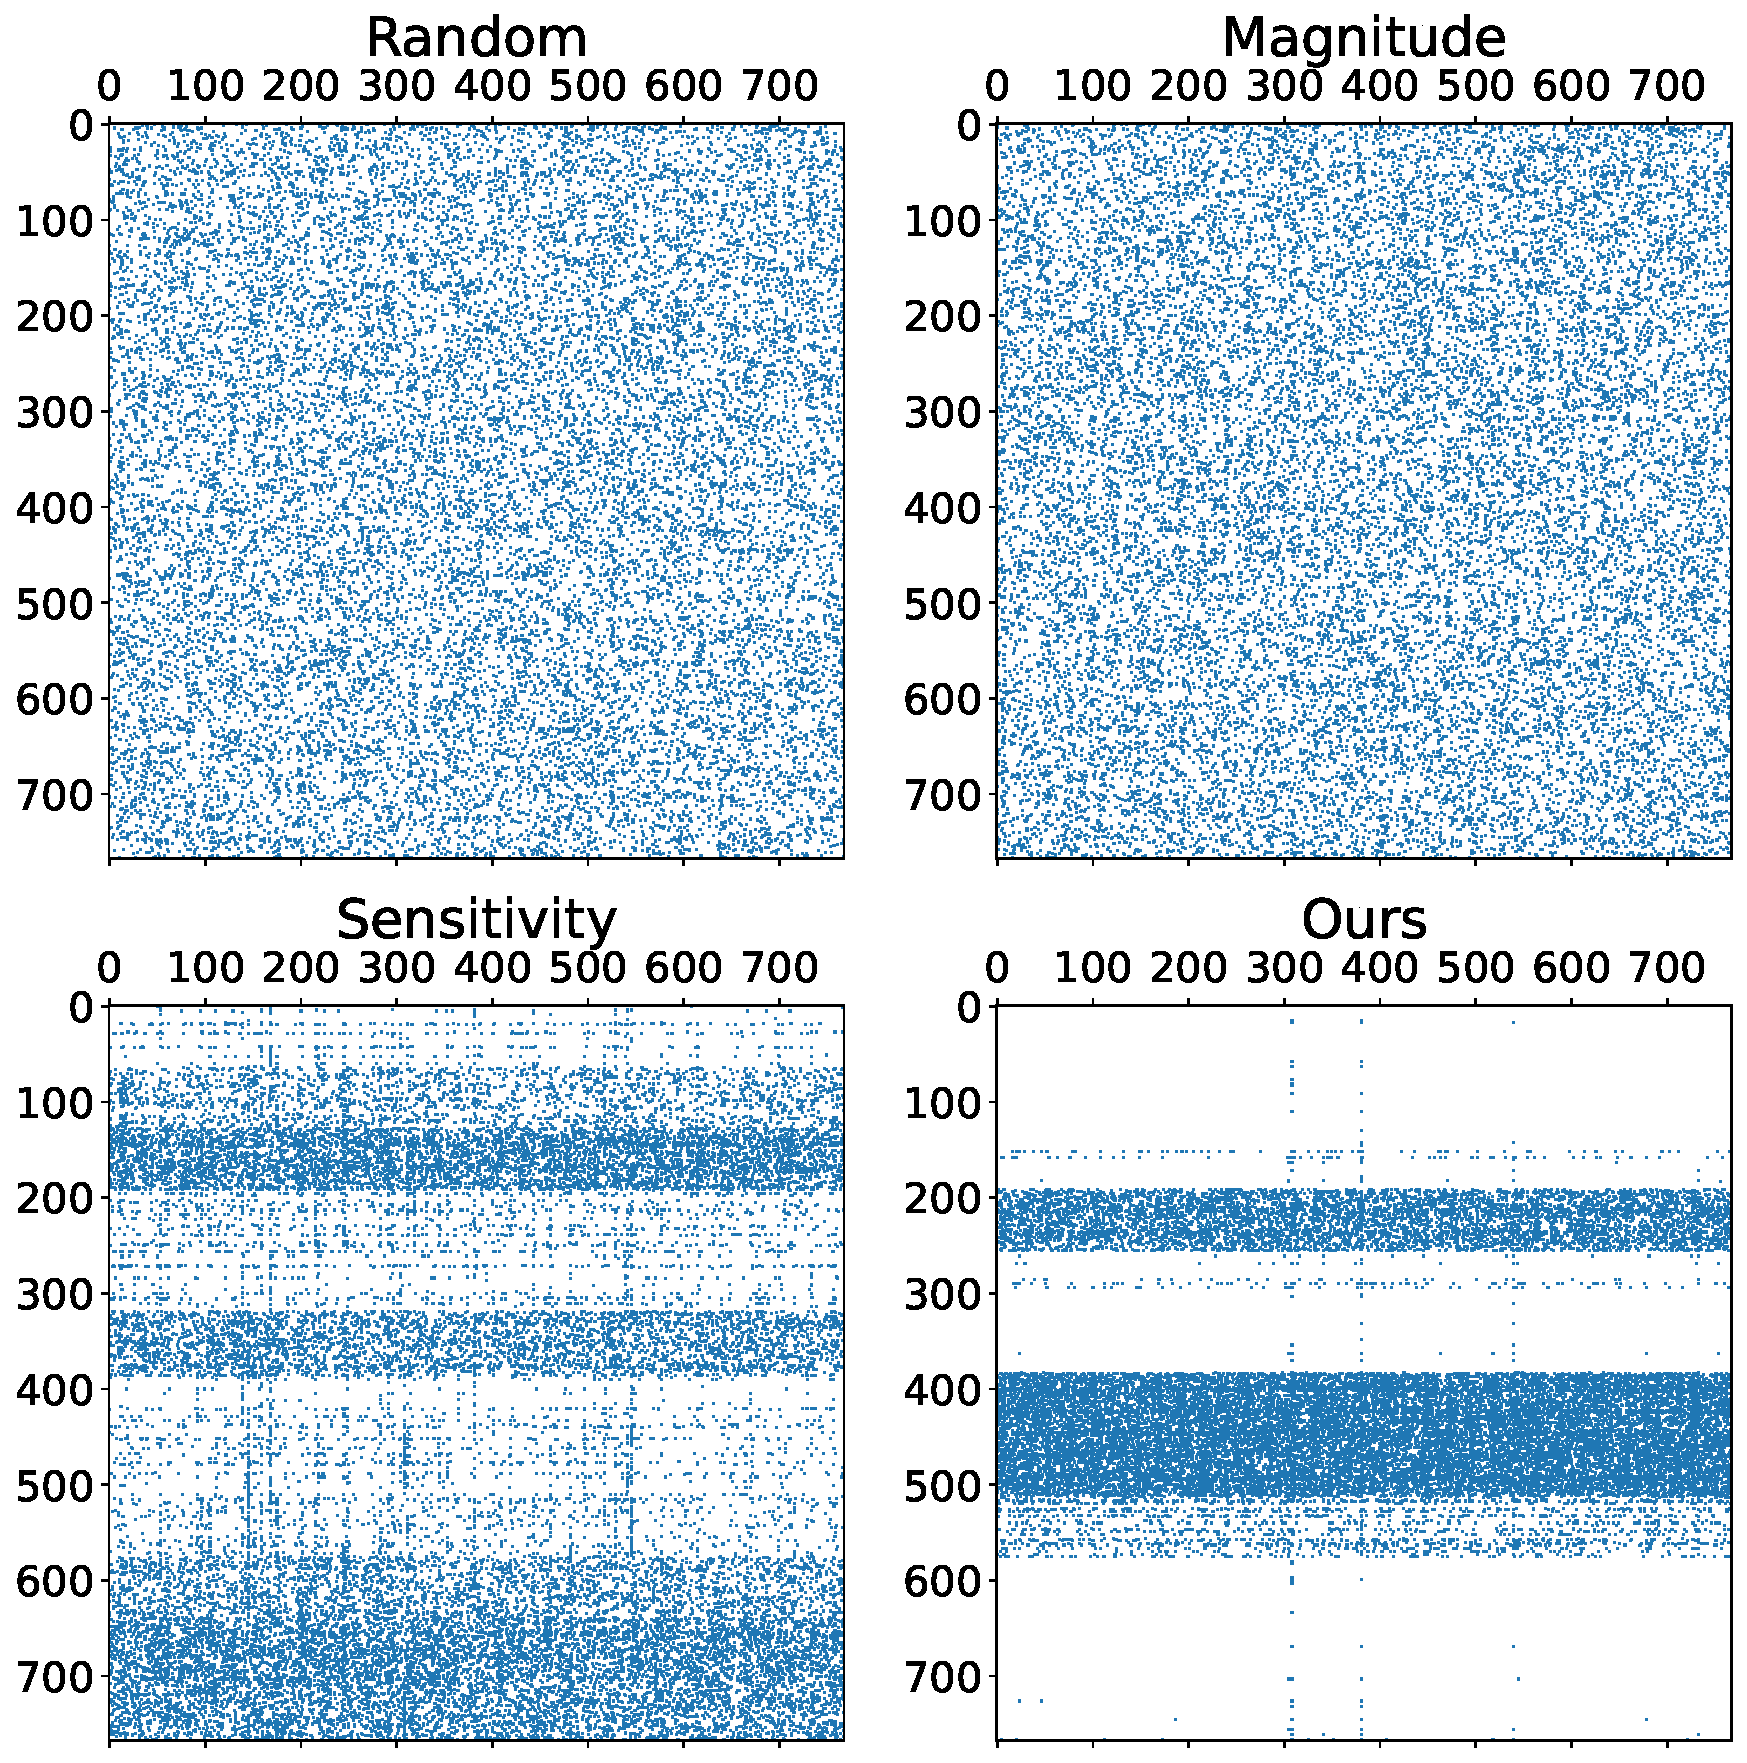
\includegraphics{./figures/sparsity_pattern_Pruning_2.pdf}}
	\caption{Sparsity pattern~(80\%) of the same weight matrix in BERT$_{\text{base}}$ trained on SST-2. See Appendix \ref{sec:C} for more details on the matrix rank distribution.}
	\label{fig:sp}
\end{figure}

\begin{figure}[t]
	\centering
	\scalebox{0.31}{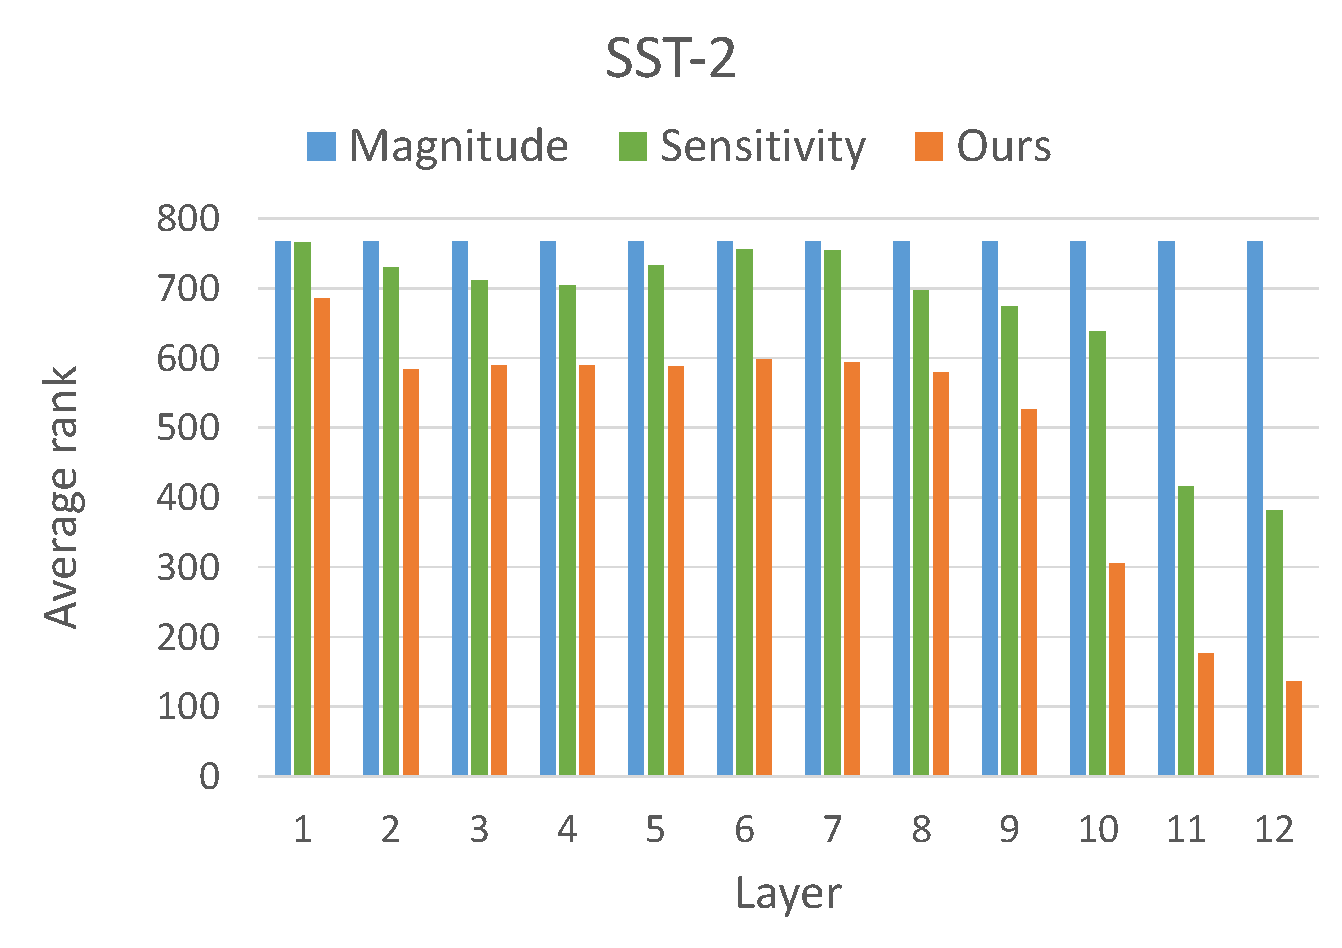
\includegraphics{./figures/rank_dist_final.pdf}}
	\caption{Layerwise distribution of average matrix rank in BERT$_{\text{base}}$ pruned  at 80\% sparsity on  SST-2.}
	\label{fig:intersim}
\end{figure}

\paragraph{Layerwise rank distribution} 
The highly structured sparsity pattern generated by  PINS intrigues our interest to further analyze the intrinsic property of parameter matrices after pruning. Specifically, we inspect the matrix rank as it is usually associated with the complexity of matrix. To this end, we visualize the layerwise rank distribution of  BERT$_{\text{base}}$ pruned using different importance criteria on SST-2 dataset. As shown in \figref{fig:intersim}, magnitude pruning produces sparse matrices that are still near full-rank despite containing 80\% zeros. Sensitivity pruning tends to generate sparsity pattern with lower rank compared to magnitude pruning. Notably, model pruned by PINS shows consistently lower matrix rank than the other two criteria. This implies that PINS is more effective at identifying the low-dimensional task representation during adaptation, which is usually correlated with tighter generalization bounds~\cite{compressionbounds,intrinsicdimension}.

\paragraph{Empirical validation of importance criterion}
In \secref{sec:analysis} we prove that the pruning decision derived by our importance criterion is theoretically optimal. Here we empirically validate this point by visualizing the change of learning objective as pruning proceeds. \figref{fig:lo} illustrates that our importance criterion indeed leads to the most significant decrease in the learning objective compared to heuristical ones like magnitude and sensitivity.
%\KZ{If every step we take at PINS is optimal, then how come the orange line
%also bumps up sometimes, instead of monotonically downward?}
%\begin{figure}[t]
%	\centering
%	\scalebox{0.3}{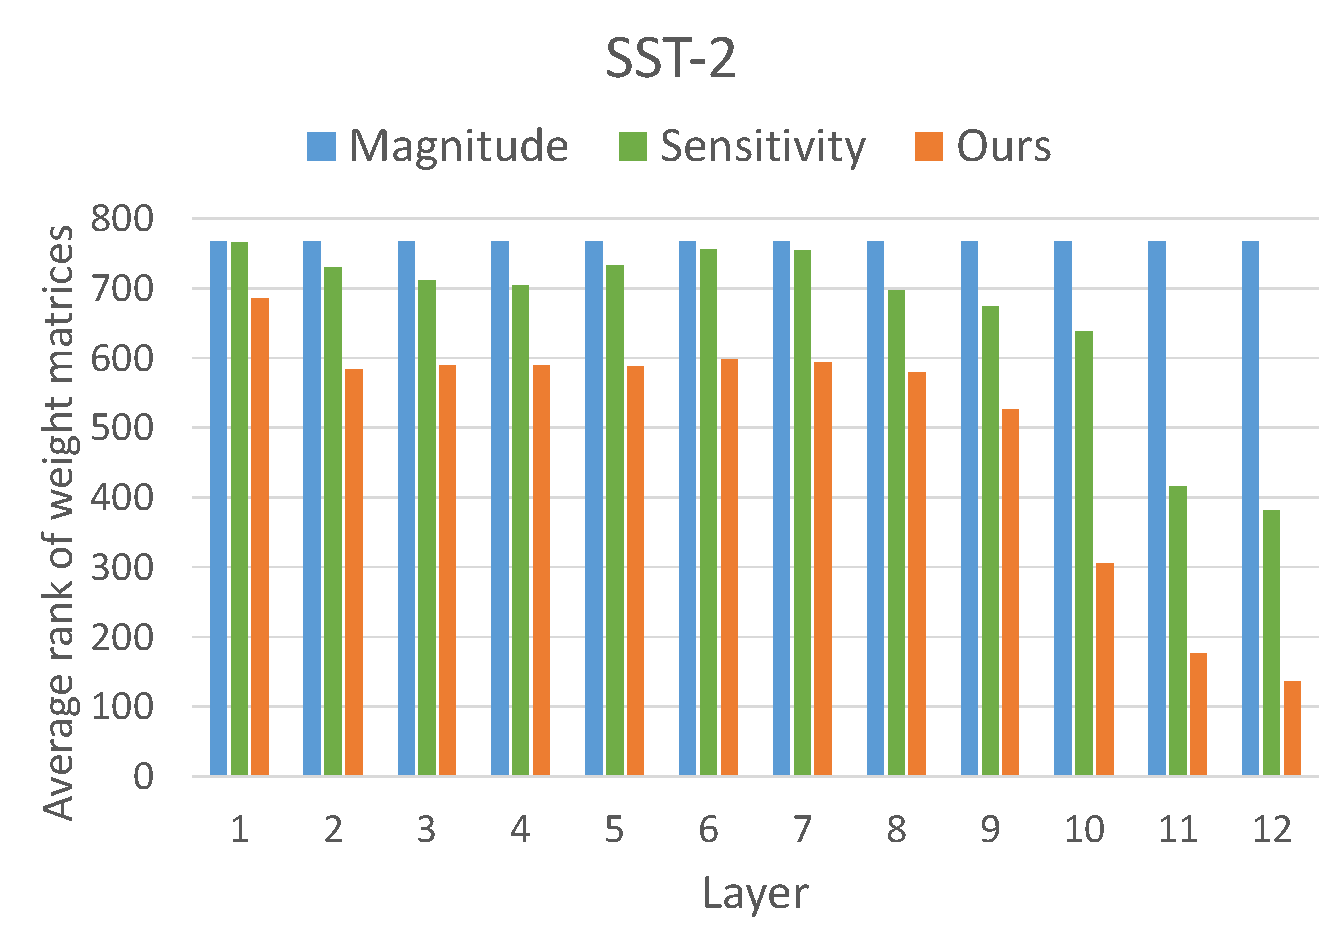
\includegraphics{./figures/rank_dist_1.pdf}}
%	\caption{Layer-wise rank distribution of weight matrices after pruning. The maximum rank is 768 for BERT$_{\text{base}}$.}
%	\label{fig:rdist}
%\end{figure}



\begin{figure}[t]
	\centering
	\scalebox{0.31}{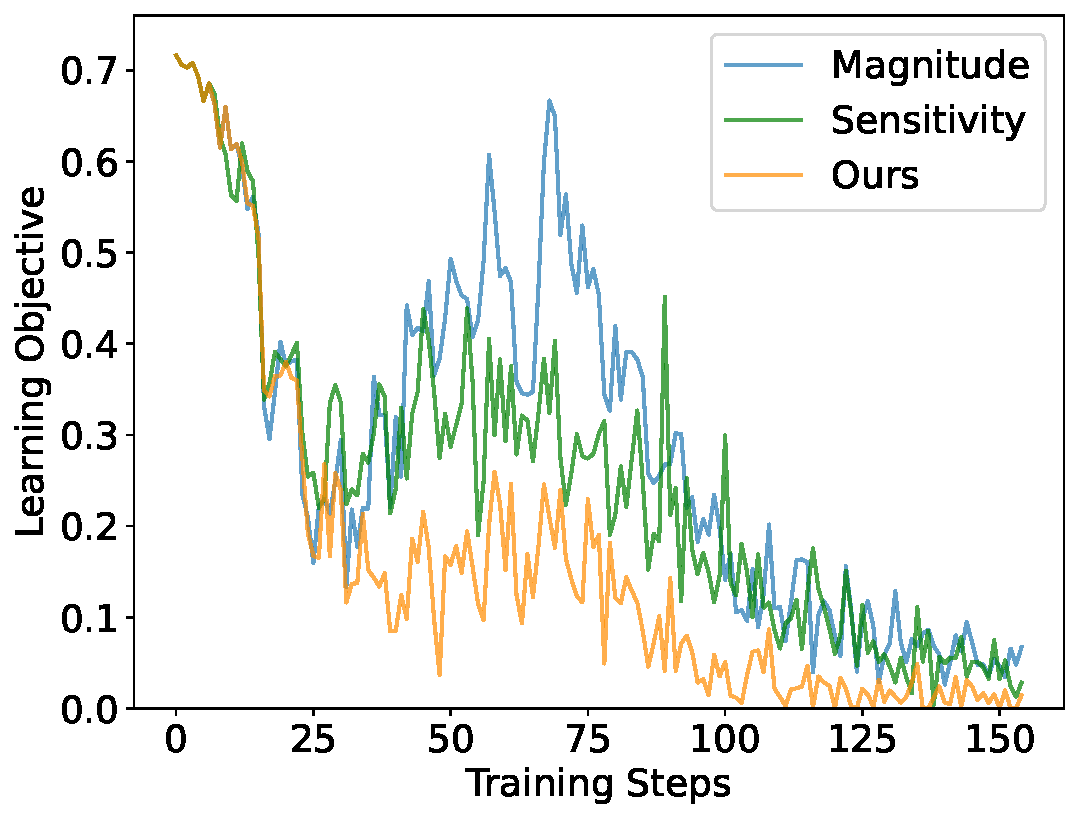
\includegraphics{./figures/LearningObjective.pdf}}
	\caption{Change of learning objective~(cross-entropy) during iterative pruning on SST-2.}
	\label{fig:lo}
\end{figure}

\begin{table}[t]
	\centering
	\small
	\begin{tabular}{c|cc|c}
		\toprule
		Sparsity & Time(s) & Storage(MB) & Acc. \\
		\midrule
		0\%      & 0.110~(1.0x)          & 340~(1.0x)  &  69.3\\
		80\%     & 0.041~(2.7x)          & 38~(8.9x) & 69.0 \\
		\bottomrule
	\end{tabular}
\caption{Practical time and storage efficiency gain on RTE with Deepsparse and CSR format. Inference is perform on Intel Xeon E5-2640 CPU with batch size 1.}
\label{table:eg}
\end{table}
\subsection{Efficiency Gain}
We can exploit the resulting high sparsity to attain practical efficiency gain on storage and inference speed. We first apply quantization  upon the pruned model and transform it into INT8 data type before saving it using Compressed Sparse Row~(CSR) format. We then leverage a sparsity-aware runtime~\cite{deepsparse} for accelerating inference. As shown in \tabref{table:eg}, on the RTE dataset, the disk space and inference time of BERT$_{\text{base}}$ pruned at 80\% sparsity can be reduced by roughly 8.9x and 2.7x respectively with negligible accuracy loss.
